\documentclass[12pt,a4paper]{article}%
\usepackage[T1]{fontenc}%
\usepackage[utf8]{inputenc}%
\usepackage{lmodern}%
\usepackage{textcomp}%
\usepackage{lastpage}%
\usepackage{graphicx}%
%
\title{Reporte Médico de Cáncer Cerebral}%
\author{Hospital XYZ}%
\date{\today}%
%
\begin{document}%
\normalsize%
\maketitle%
\newpage%
\section{Información del Paciente}%
\label{sec:InformacindelPaciente}%
\begin{tabular}{ll}%
\textbf{Nombre:}&Juan Pérez\\%
\textbf{Edad:}&45\\%
\textbf{Género:}&Masculino\\%
\textbf{ID del Paciente:}&123456\\%
\end{tabular}

%
\section{Diagnóstico}%
\label{sec:Diagnstico}%
El paciente presenta una masa en el lóbulo frontal izquierdo, indicativa de un posible glioma. Se recomienda seguimiento y biopsia para confirmar el diagnóstico.

%
\section{Imágenes de Resonancia Magnética}%
\label{sec:ImgenesdeResonanciaMagntica}%


\begin{figure}[h!]%
\centering%
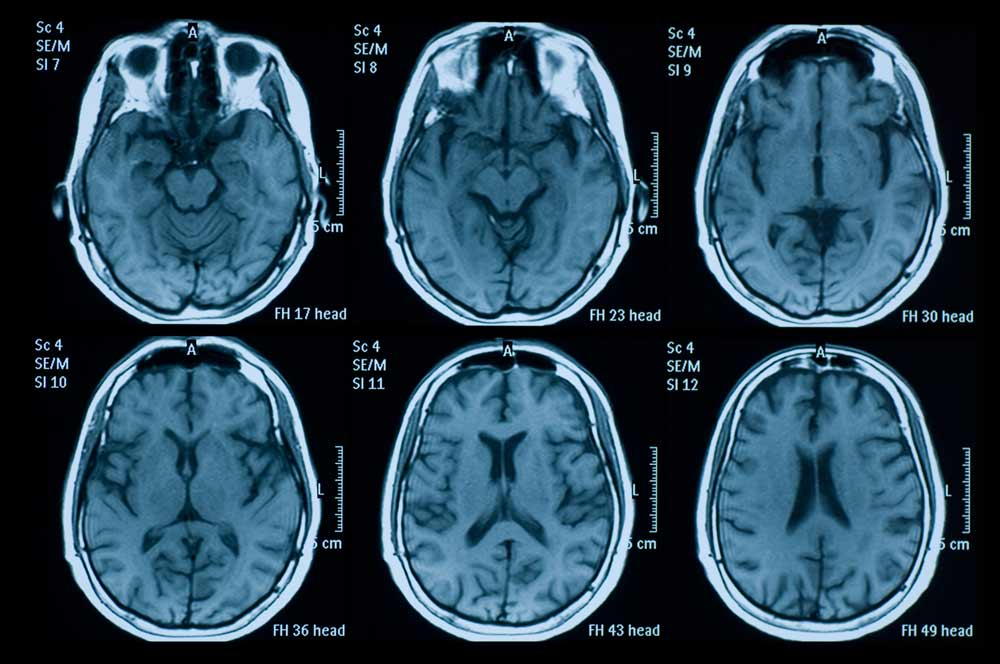
\includegraphics[width=0.8\textwidth]{C:/Users/lcres/PycharmProjects/Flask Server Brain Tumor/tumor.jpg}%
\caption{Resonancia Magnética}%
\end{figure}

%


\begin{figure}[h!]%
\centering%
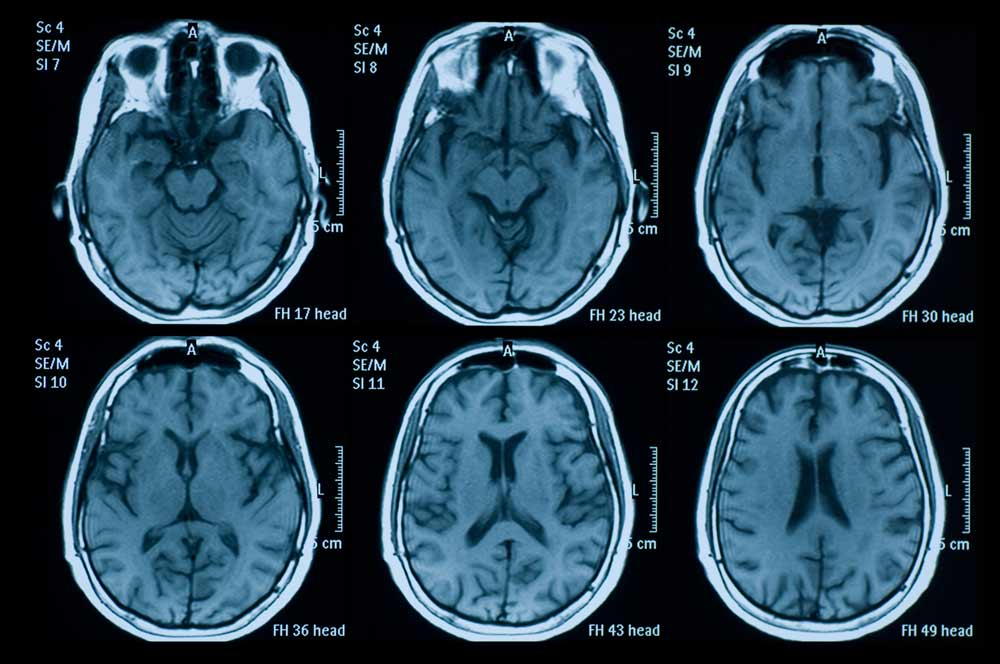
\includegraphics[width=0.8\textwidth]{C:/Users/lcres/PycharmProjects/Flask Server Brain Tumor/tumor.jpg}%
\caption{Resonancia Magnética}%
\end{figure}

%
\section{Predicciones del Modelo}%
\label{sec:PrediccionesdelModelo}%
\subsection{Imagen: tumor 1}%
\label{subsec:Imagentumor1}%
Predicción: Positivo para tumor cerebral

%
\subsection{Imagen: tumor 2}%
\label{subsec:Imagentumor2}%
Predicción: Negativo para tumor cerebral

%
\end{document}